\section{Energy resolution boost}
\label{Result}
Assume the number of expected photons $N$ on PMT obeys Poisson distribution $\pi~(\mu_N)$. Energy $E$ of Event proportional to $N=k\eta E$, in which $k$ is a factor that is relate to light yield and light transportation. The photon detection efficiency of PMT is $\eta$ and the single PE charge distribution is Gaussian distribution $G(\mu_C,\sigma_C^2)$. The output charge distribution $C$ is a hierachical model and the expectation and variance are
\begin{align}
    E[C]&=\mu_N\mu_C\\
    Var[C]&=\mu_C^2\mu_N+\mu_N\sigma_C^2
\end{align}

To be convenience, $N$ is estimated as $\hat{N}=\frac{C}{\mu_C}$ and $E$ is estimated as $\hat{E}=\frac{\hat{N}}{k}$. For  energy $E$ of events, the reconstructed energy resolution is 
\begin{equation}
    \frac{\sqrt{Var[\hat{E}]}}{E[\hat{E}]}=\frac{\sqrt{\mu_c^2\mu_N+\mu_N\sigma_c^2}}{\mu_N\mu_c}=\frac{\sqrt{1+(\frac{\sigma_c}{\mu_c})^2}}{\sqrt{\mu_N}}=\frac{\sqrt{1+(\frac{\sigma_c}{\mu_c})^2}}{\sqrt{k\eta E}}
\end{equation}

The energy resolution is dominated by the resolution of total charge of sigle PE $\mathrm{Res}$ and PDE. $\frac{\sqrt{1+(\frac{\sigma_c}{\mu_c})^2}}{\sqrt{\eta}}$ shows the energy resolution and is calculated for reference PMT and MCP-PMTs shown in Fig.~\ref{fig:EnergyResolution}. Although there exists a long tail in the charge distribution of MCP-PMT, the relative PDE of MCP-PMT is better than that of reference PMT, leading to a better energy resolution with about 0.1 boosts. Advanced waveform analysis method which models the charge distribution may eliminate the impact of long tail in charge distribution and gives a better energy resolution.
\begin{figure}[!htbp]
    \centering
    \includegraphics[width=0.5\textwidth,page=14]{figures/result/compare.pdf}
    \caption{Energy resolution as a function of the resolution of total charge and the relative PDE. The relative PDE of reference PMT is 1.}
    \label{fig:EnergyResolution}
\end{figure}